\section{Two Level Logic Synthesis Optimization}
We distinguish between sequential and combinational circuits, whose behaviour can be captured by finite-state machine state diagrams or by Boolean functions and relations. Often, sequential and combinational circuits are represented conveniently by mixed structural/behavioural models, such as  \textit{logic networks}. The goal of logic-level synthesis and optimization is to determine the microscopic structure of a circuit, i.e., its gate-level representation. \\
This chapter deals with the optimization of combinational logic circuits, modeled by two-level  \textit{sum of products}  expression forms.	
\bigskip\\
The \textbf{objective} of two-level synthesis optimization are:
\begin{itemize}
	\item Minimization of the area
	\item Optimization of performance(\textit{I/O delay} for combinational circuits and \textit{register to register path} for sequential circuit).
	\item Minimize power consumption
\end{itemize}
\bigskip
To implement a given funztion we have different possibilities, infact, in this example we can obtain different value for area and delay.\\
Given $ f = pqrs $ we obtain (a) (b) (c) (d) as possible implementations:
\begin{figure}[H]
	\centering
	\begin{subfigure}[b]{0.5\textwidth}
		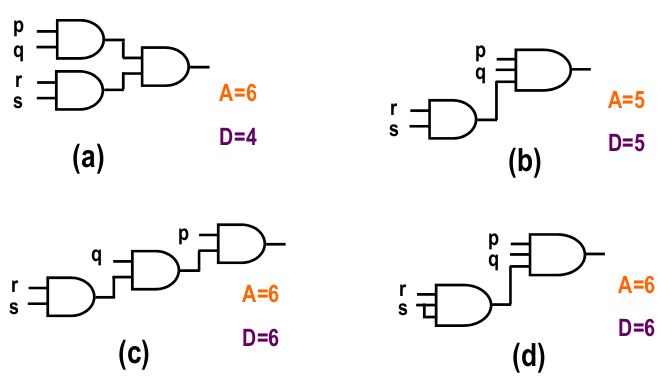
\includegraphics[width=\textwidth]{./Cap6/Images/Image1.png}
		\caption{Different Implementation}
		\label{fig:possImpl}
	\end{subfigure}
	\quad\quad
	\begin{subfigure}[b]{0.4\textwidth}
		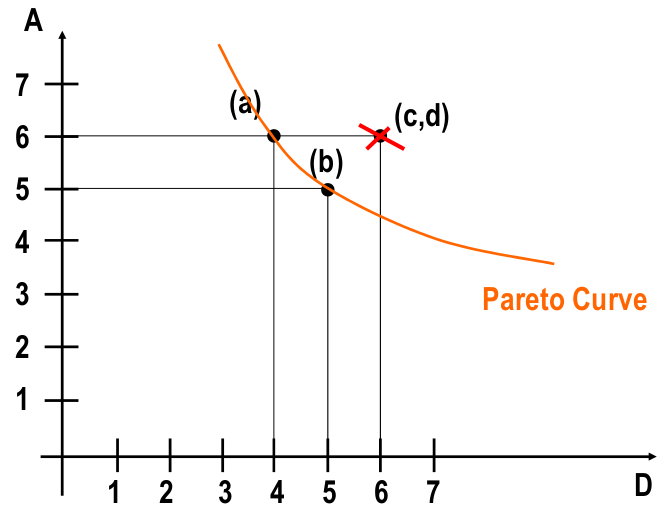
\includegraphics[width=\textwidth]{./Cap6/Images/Image2.png}
		\caption{Performance comparison}
		\label{fig:perform}
	\end{subfigure}
\end{figure}
In this case only (a) and (b) are part of pareto points, and they achieve different goal, in area or delay.
\bigskip\\
\subsection{Background and Definitions}
The \textbf{Boolean functions} we use in this case are:
\begin{itemize}
	\item \textit{Binary} Input and Output $ B = \{0, 1\} $ 
	\item \textit{Single} ( $ f : B^{n} \rightarrow B $ ) or\textit{ Multiple} (  $ f : B^{n} \rightarrow B^{m} $ ) output
	\item \textbf{Incompletely specified} so, functions \underline{with} don't care conditions ($ f: B^{n} = \{0, 1, *\} $)
\end{itemize}
\paragraph{Don't care condition}
The case in which we don't care about the value of a function, it's r\textit{related to the evirnonment} (input pattern that never occours or input patter for which some output is never observed),
\paragraph{ON-set}
Subset of the domain that make $ f = true $
\paragraph{OFF-set}
Subset of the domain that make $ f = false $
\paragraph{DC-set}
Subset of the domain for which we observe a \textit{don't care} value
\bigskip\\
For \textit{multiple output function}  ON, OFF and DC set is defined \textit{for each} component
\bigskip\\
We can give different representation that can be summarized into two categories: \textbf{visual} (Karnaugh Maps, Truth Table, Cubical Notation) or \textbf{computer oriented} (Matrices, BDDs) representations.
\begin{figure}[H]
	\centering
	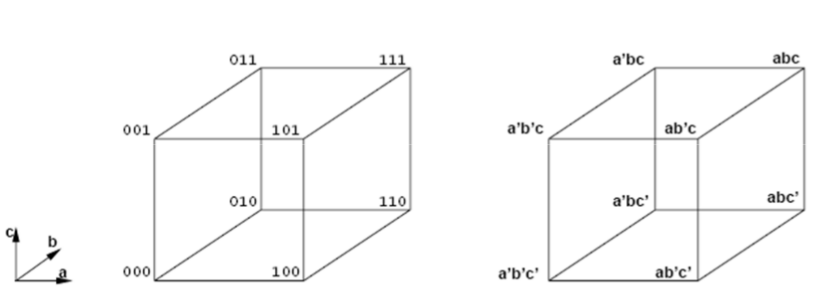
\includegraphics[width=0.6\textwidth]{./Cap6/Images/Image3.png}
	\caption{Cubical representation, in which each vertex of the cube is a minterm, can associate positional value. Example: $ ab'c \rightarrow 1_{a}0_{b}1_{c} $ \textit{(1 indicates true value)}}
	\label{fig:cubicalnotation}
\end{figure}
\paragraph{Definitions}
\begin{itemize}
	\item Boolean \textbf{variables} (\textit{Example: a, b, c, ...}) 
	\item Boolean \textbf{literals} are variables and their complement ( \textit{Example: a, a', b, b', ...})
	\item \textbf{Product or cube} is a product of literals (\textit{Example: ab'c, b'c, ...})
	\item A \textbf{Minterm} is product of \textit{all input variables} and implies a value for the function (usually 1)
	\item \textbf{Implicant} is a product (\textit{not mandatory to contain all the input variables}) that implies a value for the function (usually 1)
\end{itemize}
\paragraph{Tabular Representation}: define a truth ttable with the list of all minterm of a given function, and define a \textbf{cover} also called \textbf{implicant table} that is a list of all the implicant sufficient to define the function (\textit{Note}: implicant table is generally smaller in size than the truth table of the same function)

\begin{center}
	
	\begin{tabular}{|c|c|}
		\hline
		abc & xy \\ \hline
		000 & 00 \\ \hline
		001 & 10 \\ \hline
		010 & 00 \\ \hline
		011 & 11 \\ \hline
		100 & 00 \\ \hline
		101 & 01 \\ \hline
		110 & 11 \\ \hline
		111 & 11 \\ \hline 
	\end{tabular}
	\quad
	\quad
	\quad
	\quad
	\quad
	\quad
	\quad
	\begin{tabular}{|c|c|}
		\hline
		abc & xy \\ \hline
		001 & 10 \\ \hline
		*11 & 11 \\ \hline
		101 & 01 \\ \hline
		11* & 11 \\ \hline 
	\end{tabular}
	
	\bigskip
	Complete \textit{truth table} for $ x= ab + a'c $ and $ y = ab + bc+ ac $ (left side) and \textit{implicant table} (right side)
\end{center}
\paragraph{Logic Synthesis Problem} are related to the \textbf{implementation styles} (PLA macro-cells for \textit{two level circuits} and cell/array based for \textit{multi-level circuits}) and to the \textbf{operation mode} of the circuit (combinational, syncronous sequential or asyncronous sequential).

\subsection{Optimization for two-level circuits}
The reason why we invest so much time to the two level logic optimization are:

\begin{itemize}
	\item \textbf{Reduction} in the size of the representation
	\item \textbf{Direct implementation} of standard operating procedures (PLAs reduce size and delay).
	\item \textbf{implementation styles} based on Multi-Level nets
\end{itemize}

\subsubsection{Programmable Logic Arrays}
PLas are macro-cells with rectangular structure that implement any multi-output function. Their layout is generated by module generators and it's very popular in the '70/'80 but they are still used in some modern application, such as smart controllers, and in emerging technologies (Graphene, Crossbar Latch). They have some \textbf{advantages} as simplicity and predictable timing, but also the \textbf{disadvantages} of not much flexibility (with respect to cell based realization)
\paragraph{Graphene PLAs} are an open topic for researcher because there are interesting features of the graphene that allow us to recreate a complex function with a very low usage of gates (and so better performance and less area utilization)

\subsubsection{Approaches of Two-level Optimization}
Assuming that all implicants have the same cost, our goals are, the \textit{reduction of the number of implicants and literals}, infact implicants correspond to a PLA rows and literals to transistors.

\paragraph{Minimum cover} is the cover of a function with the \textit{minimum} number of implicants (\textbf{Global Optimum})

\paragraph{Minimal or irreduntant cover} is a cover that isn't a superset of another one (\textit{no implicant can be dropped}) and correspond to \textbf{local optimum}.

\paragraph{Minimal with respect to 1 implicant containment} cover in which no implicant is contained by another one (\textbf{weak local optimum})

Given this definition we can use \textit{exact methods} to compute \textit{\underline{minimum cover}} (often difficult/impossible for large function) or \textit{\underline{}} to compute \textit{\underline{minimal cover}}

\begin{itemize}
	\item \textbf{Exact Methods} are based on Quine's theorem (Quine-McCluskey, Petrick's methos, Espresso exact)
	\item \textbf{Heuristic Methods} MINI, PRESTO, ESPRESSO and so on.
\end{itemize}
Considering all possible implicant, we define some subset with some characteristics:
\begin{itemize}
	\item \textbf{Prime implicant}, implicant \textit{not} contained or covered by any other implicant
	\item \textbf{Prime cover} a cover in which \textit{all} implicants are prime
	\item \textbf{Essential Prime implicants} covers a minterm \textit{not} covered by any one else. They \textit{needs} to be included into the cover 
\end{itemize}
\subsubsection{Exact Logic Minimization}
The most used algorithms are based on \textit{Quine's theorem} that says:
\begin{center}
	\textit{There is a minimum cover that is prime}\\
\end{center}
and as consequence of this theorem we restrict our search of minimum cover only to prime implicants; for this reason the Quine-Based methods:
\begin{enumerate}
	\item Compute the prime implicants
	\item Determine the minimum cover
\end{enumerate} 
All the exact methods need the\textit{ primes table as starting point}, so that the optimization problem is reduced to a covering problem.\\
Considering a completely specified single-output functions, a \textbf{prime implicant table} is a binary-valued matrix $A$ whose columns are in one-to-one correspondence with the prime implicants of the function $f$ and whose rows are in one-to-one correspondence with its minterms.\\ 
A minimum cover is a minimum set of columns which covers all rows, or equivalently a minimum set of primes covering all minterms. Therefore the covering problem can be viewed as the problem of finding a binary vector $x$ representing a set of primes with minimum cardinality $|x|$ such that:
\begin{center}
	$Ax \geqslant \textbf{1}$
\end{center}
where \textbf{1} is the "unary vector" and as $x$ match he number of minterms and primes.

\paragraph{Example} given the function $ f= a'b'c' + a'b'c + ab'c + abc + abc' $
\bigskip\\

\begin{center}
	
	\begin{tabular}{|c|c|c|}
		\hline
		$\alpha$ & 00* & 1 \\ \hline
		$\beta$ & *01 & 1 \\ \hline
		$\gamma$ & 1*1 & 1 \\ \hline
		$\delta$ & 11* & 1 \\ \hline
	
	\end{tabular}
	\quad
	\quad
	\quad
	\quad
	\begin{tabular}{|c|c c c c|}
		\hline
		 {} & $\alpha$ & $\beta$ & $\gamma$ & $\delta$ \\ \hline
		 000 & 1 & 0 & 0 & 0 \\ \hline
		 001 & 1 & 1 & 0 & 0 \\ \hline
		 101 & 0 & 1 & 1 & 0 \\ \hline
		 111 & 0 & 0 & 1 & 1 \\ \hline
		 110 & 0 & 0 & 0 & 1 \\ \hline
		 
	\end{tabular}

	\bigskip
	
	\textit{Primes} to the left side, \textit{Prime table} to the right side
\end{center}

Then use the $x$ vector multiplied by $A$ to compute if all the implicant are covered, so:

\begin{center}
	
	\begin{tabular}{ c c }
	
		\begin{tabular}{|c c c c|}
			
			1 & 0 & 0 & 0 \\
			1 & 1 & 0 & 0 \\ 
			0 & 1 & 1 & 0 \\ 
			0 & 0 & 1 & 1 \\ 
			0 & 0 & 0 & 1 \\ 

			
		\end{tabular}
		
	\quad
	\quad
	
		\begin{tabular}{|c|}
			
			$x_{\alpha}$ \\
			$x_{\beta}$ \\
			$x_{\gamma}$ \\
			$x_{\delta}$ \\
			
		\end{tabular}
		
	\end{tabular}
	\bigskip
	
	Assigning to $x_{\alpha}, x_{\beta} ... $ value 1 only if it's considered part of the cover, then try to remove one of them from the cover and recompute if $Ax \geqslant \textbf{1}$, repeat this until find the \textit{minimum cover}.
\end{center}
\paragraph{Covering Problem} is a \underline{NP-hard problem} due to:
\begin{itemize}
	\item Columns - prime implicants (Up to $3^{n}/3$)
	\item Rows - minterms ($2^{n}$).
	\item Selection Boolean vector for primes $x$ and determine it such that $Ax \geqslant \textbf{1}$ 
	\item Select at the same time \textit{enough columns} to cover all rows and \textit{minimize the cardinality} of $x$.
\end{itemize}
\subsection{Quine-McCluskey}
The method involves two steps:
\begin{enumerate}
	\item Finding all prime implicants of the function.
	\item Use those prime implicants in a prime implicant chart to find the essential prime implicants of the function, as well as other prime implicants that are necessary to cover the function.
\end{enumerate} 
\paragraph{Example} Given the function $ f(x,y,z,v) = \Sigma m(1,4,5,6,7,9,11,14,15) $ so that the function will be equal to 1 for the values specified (1,4,5,6...), in the following step we attempt reduction and merge some minterms wher their \textit{mindistance  = 1}

\begin{center}
  
\begin{tabular}{ c c }
	
	\begin{tabular}{|c c c c|c c|}
		\hline
		x & y & z & v & res & val \\ \hline
		0 & 0 & 0 & 0 & 0 & {} \\ 
		0 & 0 & 0 & 1 & 1 & \textbf{m1} \\
		0 & 0 & 1 & 0 & 0 & {} \\
		0 & 0 & 1 & 1 & 0 & {} \\
		0 & 1 & 0 & 0 & 1 & \textbf{m4} \\
		0 & 1 & 0 & 1 & 1 & \textbf{m5} \\
		0 & 1 & 1 & 0 & 1 & \textbf{m6} \\
		0 & 1 & 1 & 1 & 1 & \textbf{m7} \\
		1 & 0 & 0 & 0 & 0 & {} \\
		1 & 0 & 0 & 1 & 1 & \textbf{m9} \\
		1 & 0 & 1 & 0 & 0 & {} \\
		1 & 0 & 1 & 1 & 1 & \textbf{m11} \\
		1 & 1 & 0 & 0 & 0 & {} \\
		1 & 1 & 0 & 1 & 0 & {} \\
		1 & 1 & 1 & 0 & 1 & \textbf{m15} \\	
		1 & 1 & 1 & 1 & 1 & \textbf{m14} \\ \hline
	\end{tabular}
	
	\quad
	\quad
	\quad
	
	\begin{tabular}{|c c c c c |c|}
		\hline
		{} & x & y & z & v & {} \\ \hline
		m1 & 0 & 0 & 0 & 1 & \checkmark \\ 
		m4 & 0 & 1 & 0 & 0 & \checkmark  \\
		m5 & 0 & 1 & 0 & 1 & \checkmark  \\
		m6 & 0 & 1 & 1 & 0 & \checkmark  \\
		m7 & 1 & 1 & 1 & 1 & \checkmark  \\
		m9 & 1 & 0 & 0 & 1 & \checkmark  \\
		m11 & 1 & 0 & 1 & 1 & \checkmark  \\
		m14 & 1 & 1 & 1 & 0 & \checkmark   \\
		m15 & 1 & 1 & 1 & 1 & \checkmark  \\ \hline
		
		
	\end{tabular}
	
	\quad
	\quad
	\quad
	
	\begin{tabular}{|c c c c c |c|}
		\hline
		
		{} & x & y & z & v & {} \\ \hline
		m1-m5 & 0 & * & 0 & 1 & \textbf{a} \\ 
		m1-m4 & * & 0 & 0 & 1 & \textbf{b}  \\
		m4-m5 & 0 & 1 & 0 & * & \checkmark  \\
		m4-m6 & 0 & 1 & * & 0 & \checkmark  \\
		m5-m7 & 0 & 1 & * & 1 & \checkmark  \\
		m6-m7 & 0 & 1 & 1 & * & \checkmark  \\
		m6-m14 & * & 1 & 1 & 0 & \checkmark  \\
		m7-m15 & * & 1 & 1 & 1 & \checkmark   \\
		m9-m11 & 1 & 0 & * & 1 & \textbf{c}  \\
		m11-m15 & 1 & 1 & 1 & * & \checkmark  \\ 
		m14-m15 & 1 & * & 1 & 1 & \textbf{d}  \\ \hline
		
	\end{tabular}
	
	\end{tabular}
	

	
	\begin{tabular}{|c c c c c |c|}
		\hline
		
		{} & x & y & z & v & {} \\ \hline
		m4-m5-m6-m7 & 0 & 1 & * & * & \textbf{e} \\ 
		m6-m7-m14-m15 & * & 1 & 1 & * & \textbf{f}  \\ \hline
		
	\end{tabular}

\end{center}
\bigskip
In this case \textbf{a, b, c, d, e, f} are implicant included into the cover because cannot be merged.\\
Now we have to identify the \textbf{essential prime implicants} and include it into the cover. To identify the essential we have to check if that implicant is the only one that cover \textit{a minterm}, in that case it's essential and has to be part of the cover.





\begin{center}
	
	\begin{tabular}{|c| c c c c c c|}
		\hline
		{} & a & b & c & d & \textbf{e} & \textbf{f} \\ \hline
		m1 & 1 & 1 & {} & {} & {} & {} \\
		m4 & {} & {} & {} & {} & \underline{\textbf{1}} & {} \\
		m5 & 1 & {} & {} & {} & 1 & {} \\
		m6 & {} & {} & {} & {} & 1 & 1 \\
		m7 & {} & {} & {} & {} & 1 & 1 \\
		m9 & {} & 1 & 1 & {} & {} & {} \\
		m11 & {} & {} & 1 & 1 & {} & {} \\
		m14 & {} & {} & {} & {} & {} & \underline{\textbf{1}} \\
		m15 & {} & {} & {} & 1 & {} & {} \\ \hline
		
	\end{tabular}
	
\bigskip
In this case \textit{e and f} are essential because they are the only that covers m4 (covered by e) and m14 (covered by f). Selecting these two implicans we have to consider all the minterms covered already by these. After that we can chose the prime implicants that are not essential. The only minterms that remain uncovered are: m1, m9, m11.

	\begin{tabular}{|c| c c c c |}
		\hline
		{} & a & \textbf{b} & \textbf{c} & d  \\ \hline
		m1 & 1 & 1 & {} & {} \\
		m9 & {} & 1 & 1 & {} \\
		m11 & {} & {} & 1 & 1 \\ \hline
	
	\end{tabular}
\bigskip

The final cover will be \textbf{ e, f, b, c } so that $f = yz + x'y + y'z'v + xy'v$ 

\end{center}

\subsection{Petrick's Method}




